\documentclass[9pt,a4paper]{extarticle}
\usepackage[utf8]{inputenc}
\usepackage[T1]{fontenc}
\usepackage[spanish]{babel}
\usepackage{lmodern,microtype,graphicx,xcolor,geometry,titlesec,hyperref}
\geometry{top=11mm,bottom=11mm,left=13mm,right=13mm}
\definecolor{navy}{HTML}{18324F}
\definecolor{teal}{HTML}{147D86}
\hypersetup{colorlinks=true,urlcolor=teal,pdftitle={Frontier Agent - Systems design},pdfauthor={Equipo Frontier Agent}}
\pagestyle{empty}
\setlength{\parindent}{0pt}
\setlength{\parskip}{3pt}
\setlength{\emergencystretch}{1em}
\titleformat{\section}{\color{navy}\bfseries\fontsize{10}{11}\selectfont}{}{0pt}{}
\titlespacing*{\section}{0pt}{6pt}{2pt}
\begin{document}
{\color{navy}\bfseries\fontsize{20}{22}\selectfont Frontier Agent}\hfill{\color{teal}\bfseries RETO 1}

{\color{navy}\fontsize{10}{12}\selectfont Operación visual de aplicaciones desconocidas}\hfill{\small Systems design | v0.7}

\vspace{2pt}{\color{teal}\hrule height 1pt}\vspace{5pt}
\section{Problema, alcance y supuestos}
Ejecutar tareas por píxeles y entrada VNC en apps nunca vistas: cambios exactos, sin duplicados ni acciones adicionales, con resultado veraz. El evaluador entrega escritorio por tarea y lo resetea a los cinco minutos. Leer dimensiones y fecha de la app. Modelo visual permitido y concurrencia aún por validar. Excluimos DOM/API internos, archivos remotos y entrenamiento por aplicación: solo hay acceso visual. El agente no recibe respuestas esperadas ni usa reset/check en evaluación.

\section{Arquitectura, memoria y trazabilidad}
FastAPI/Pydantic autentica y acepta en menos de dos segundos. PostgreSQL conserva tareas, resultados e interacciones; SQLAlchemy asíncrono/psycopg y Alembic gestionan tablas propias. Tarea y outbox se confirman juntos; dispatcher publica referencias a Redis. LangGraph orquesta y persiste checkpoints por tarea con AsyncPostgresSaver; AsyncPostgresStore guarda conocimiento permitido. LangChain integra modelos/tools. Orquestador con operador, verificador y recuperador, delegados por hitos; un ejecutor valida y envía acciones por VNC directo (AsyncVNC y puente WSS, probado en notebook). Ciclo: observar, actuar y verificar. Historial por tarea/ejecución/agente, capturas privadas referenciadas; credenciales fuera del modelo y memoria de negocio aislada entre evaluaciones.

\section{Decisiones y escalabilidad}
\textbf{VNC directo} evita navegador de noVNC/Playwright; revisar licencia/mantenimiento. \textbf{API y workers separados} evitan peticiones largas, a costa de cola/coordinación. \textbf{Especialistas por hitos} separan responsabilidades frente al agente monolítico, pero añaden latencia. \textbf{PostgreSQL desde demo} evita usar la cola como único estado durable, a costa de pools/migraciones.

Demo: VPS con Compose, proxy HTTPS, API, worker, PostgreSQL, Redis y volumen; punto único de fallo. Producción: réplicas API, scheduler con cuotas, workers y gateways VNC escalables, almacenamiento privado y LangSmith. Escalar por escritorios independientes y cuota del modelo. Un ejecutor por escritorio: gateway valida propiedad/versión, workers sin VNC directo. Antes de reasignar, confirmar cierre anterior; un lease expirado no basta.

\section{Casos difíciles, fallos y límite de tiempo}
Homónimos: fallar sin modificar y explicar identificadores. Edición: preservar otros campos, seleccionar todo y verificar persistencia. Clics de 150--200 ms y espera de repintado. Consultas sin mutación; exportación con filtros verificados. Texto de pantalla no amplía el alcance. Guardado incierto: reobservar; checkpoints no hacen idempotente un clic. Supervisor independiente: bloquear acciones desde 270 s, cancelar pendientes y desconectar antes del estado terminal; cierre objetivo menor a 285 s, incluida cola. Descartar propuestas tardías; no reanudar tras reset/plazo. Evidencia insuficiente: fallar con razón; verificación visual no garantiza conocer todo el estado interno.

\section{Plan de medición y observabilidad}
E1--E5, tres repeticiones desde reset: creación, edición mínima, consulta, exportación y rechazo de homónimos. Metas: \textbf{15/15 correctas}, \textbf{3/3 rechazos} y \textbf{0} cambios extras, duplicados, falsos éxitos o secretos. Harness combina check con estado/resumen. Aceptación \textbf{<2 s}, cierre \textbf{<285 s} y acciones posteriores \textbf{0}. Preguntas: línea \texttt{respuesta:} con valor primero y dos datos separados por \texttt{;}.

Variar controles, popups, paginación y fecha; probar modelo lento, desconexión tras guardar, worker caído y propuesta vieja. Medir éxito, espera, duración, pasos, coste y cancelación con destinos independientes/compartidos. Solo transporte e interacción VNC comprobados; cifras anteriores son metas. Demo: eventos en PostgreSQL. Producción: LangSmith registra trazas filtradas por tarea/agente/tool; excluir secretos, URLs e imágenes por defecto, sin bloquear tareas. LangGraph ejecuta; LangSmith observa.
\section{Arquitectura de producción}
\begin{center}
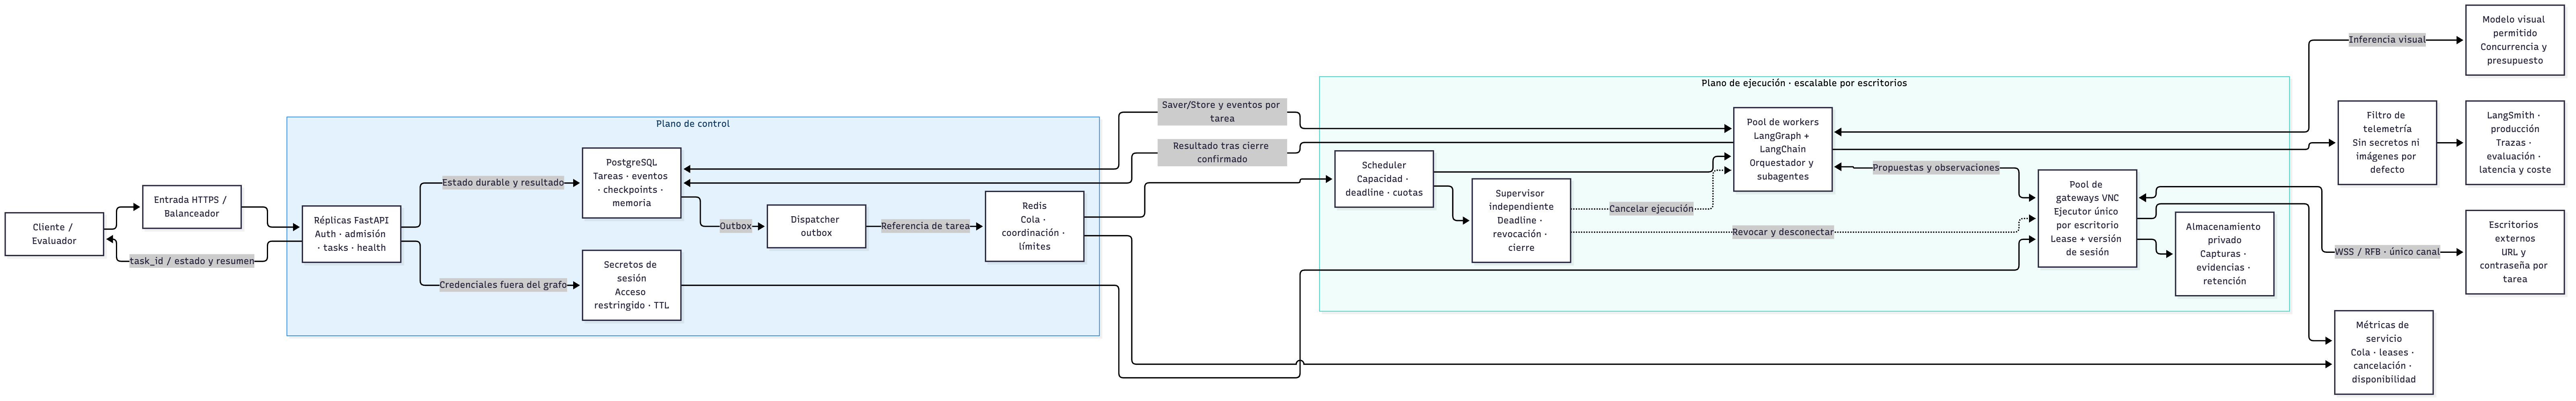
\includegraphics[width=\linewidth,height=62mm,keepaspectratio]{docs/01-systems-design/arquitectura/arquitectura-produccion.png}

{\fontsize{7.5}{9}\selectfont Arquitectura de producción exportada desde Mermaid. Imagen de alta resolución entregada también por separado.}
\end{center}
\vfill
{\color{teal}\hrule height 0.5pt}\vspace{3pt}
{\fontsize{7}{8}\selectfont\color{navy} GET /health | POST /tasks $\rightarrow$ task\_id | GET /tasks/\{id\} $\rightarrow$ estado y resumen. Bearer token en todas las llamadas.}
\end{document}
